\section{Materiales y métodos}

Para realizar este estudio, el primer pasó que se llevó a cabo fue la obtención de los genes relacionados con el fenotipo. Los descargamos de la página Human Phenotype Ontology mediante la introducción del ID del fenotipo, en nuestro caso "HP:0000526". Una vez obtenidos los genes asociados, utilizamos StringDB para analizarlos.


\subsection{STRING}


STRING es una base de datos que permite analizar y visualizar interacciones entre proteínas y genes. A continuación, se muestras los pasos llevados a cabo para obtener una red de interacción de los genes de un fenotipo concreto:

\begin{itemize}
	\item Visitamos la página de STRING
	\item Seleccionamos la opción para intnroducir multiples proteínas
	\item Introducimos solo los nombres de los genes descargados de Human Phenotype Ontology.
	\item Especificamos la especie, en este caso, Homo sapiens.
	\item STRING generará una red de interacciones, mostrando conexiones basadas en interacciones experimentales, predicciones, y bases de datos de coexpresión.
	\item Se guarda como imagen la red obtenida.
\end{itemize}

Entre los objetivos del uso de STRING están visualizar las interacciones proteicas conocidas y predichas, identificar posibles proteínas clave o "hubs" dentro de la red y evaluar la conectividad y la funcionalidad de los genes en el contexto del fenotipo elegido.
	
Tras introducir el nombre de todos los genes asociados a nuestro fenotipo obtuvimos la siguiente red de interacciones:

\newpage

\begin{figure}[h] % [h] indica que queremos la imagen aquí, en la posición actual
	\centering
	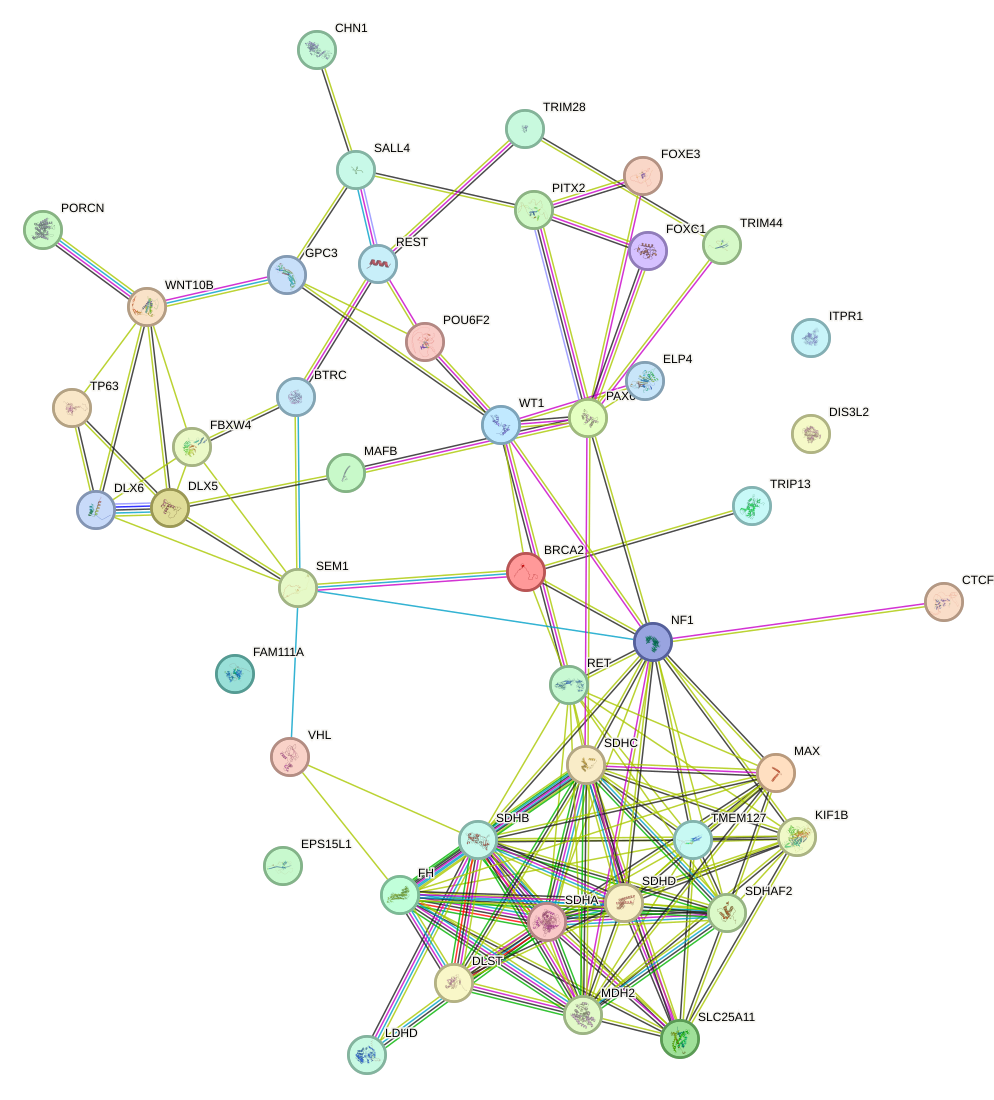
\includegraphics[width=1\textwidth]{figures/red_interaccion_aniridia.png} % Especifica la ruta y el tamaño
	\caption{Red de interacción con los genes asociados al fenotipo HP:0000526} % Agrega una leyenda si deseas
	\label{fig:mi-imagen} % Etiqueta para referenciar la imagen en el texto
\end{figure}


